\documentclass[11pt,a4paper]{article}

\usepackage[margin=1in]{geometry}
\usepackage[T1]{fontenc}
\usepackage[utf8]{inputenc}
\usepackage{lmodern}
\usepackage{graphicx}

\title{Big Data Storage and Retrieval Report}
\author{}
\date{\today}

\begin{document}
\maketitle

\section{Abstract}
This report presents the work done for the Big Data Storage and Retrieval assignment. The dataset was cleaned, modeled, and loaded into PostgreSQL, MongoDB, and Neo4j. After that, three analysis tasks were implemented. The analysis and benchmark parts were completed for PostgreSQL and MongoDB. Neo4j was modeled, but it was not used for the analysis and benchmark stages because of technical issues during the work. The results show that PostgreSQL gave more stable benchmark numbers, while MongoDB was very strong for the text search task. MongoDB query Q1 was much slower on the test laptop, so its benchmark was run only one time.

\section{Introduction}
The goal of this assignment was to compare different database models for an e-commerce dataset that contains customer events, campaigns, campaign messages, first purchase dates, and friendship links between users. The work followed three main parts from the assignment:
\begin{itemize}
    \item data modeling and storage,
    \item data analysis,
    \item benchmarking.
\end{itemize}

The cleaned dataset used in this work contains the following files:
\begin{itemize}
    \item \texttt{campaigns.csv}: 1{,}907 rows,
    \item \texttt{client\_first\_purchase\_date.csv}: 175{,}780 rows,
    \item \texttt{events.csv}: 1{,}277{,}717 rows,
    \item \texttt{friends.csv}: 1{,}974{,}234 rows,
    \item \texttt{messages.csv}: 2{,}994{,}126 rows.
\end{itemize}

The experiments were run on a laptop with Microsoft Windows 11 Pro, an Intel Core i5-9300H CPU at 2.40 GHz, 4 cores and 8 logical processors, and about 8 GB RAM. PostgreSQL and MongoDB were used locally on the machine. Neo4j was also prepared for the modeling task. The exact software version numbers were not saved in the repository during the experiments, so they are not reported here.

\section{Data Modeling}
\subsection{Data Cleaning}
The cleaning step was implemented in \texttt{scripts/clean\_data.py}. The script reads the raw CSV files and writes cleaned files to \texttt{data/processed}. The main cleaning actions were:
\begin{itemize}
    \item trimming spaces,
    \item replacing common missing tokens such as \texttt{na}, \texttt{null}, and empty strings with empty values,
    \item normalizing Boolean values into a consistent form,
    \item normalizing date and datetime fields,
    \item normalizing numeric values,
    \item skipping malformed rows with extra unnamed columns,
    \item skipping fully empty rows.
\end{itemize}

This step was important because the same cleaned files were used by all database loaders, which helped make the comparison fair.

\subsection{PostgreSQL Data Model}
The PostgreSQL model was implemented in \texttt{scripts/load\_data\_psql.sql}. A relational design was chosen because the dataset has clear entities and many relationships that fit well into tables with keys and constraints.

The main tables are:
\begin{itemize}
    \item \texttt{users},
    \item \texttt{clients},
    \item \texttt{products},
    \item \texttt{events},
    \item \texttt{campaigns},
    \item \texttt{messages},
    \item \texttt{friends}.
\end{itemize}

The loader first creates staging tables, imports the cleaned CSV files, and then fills the final tables. Primary keys, foreign keys, and a unique key on \texttt{(campaign\_id, campaign\_type)} were used to keep the data consistent. This model is normalized and easy to query with joins, which is useful for the analysis tasks.

\begin{figure}[htbp]
    \centering
    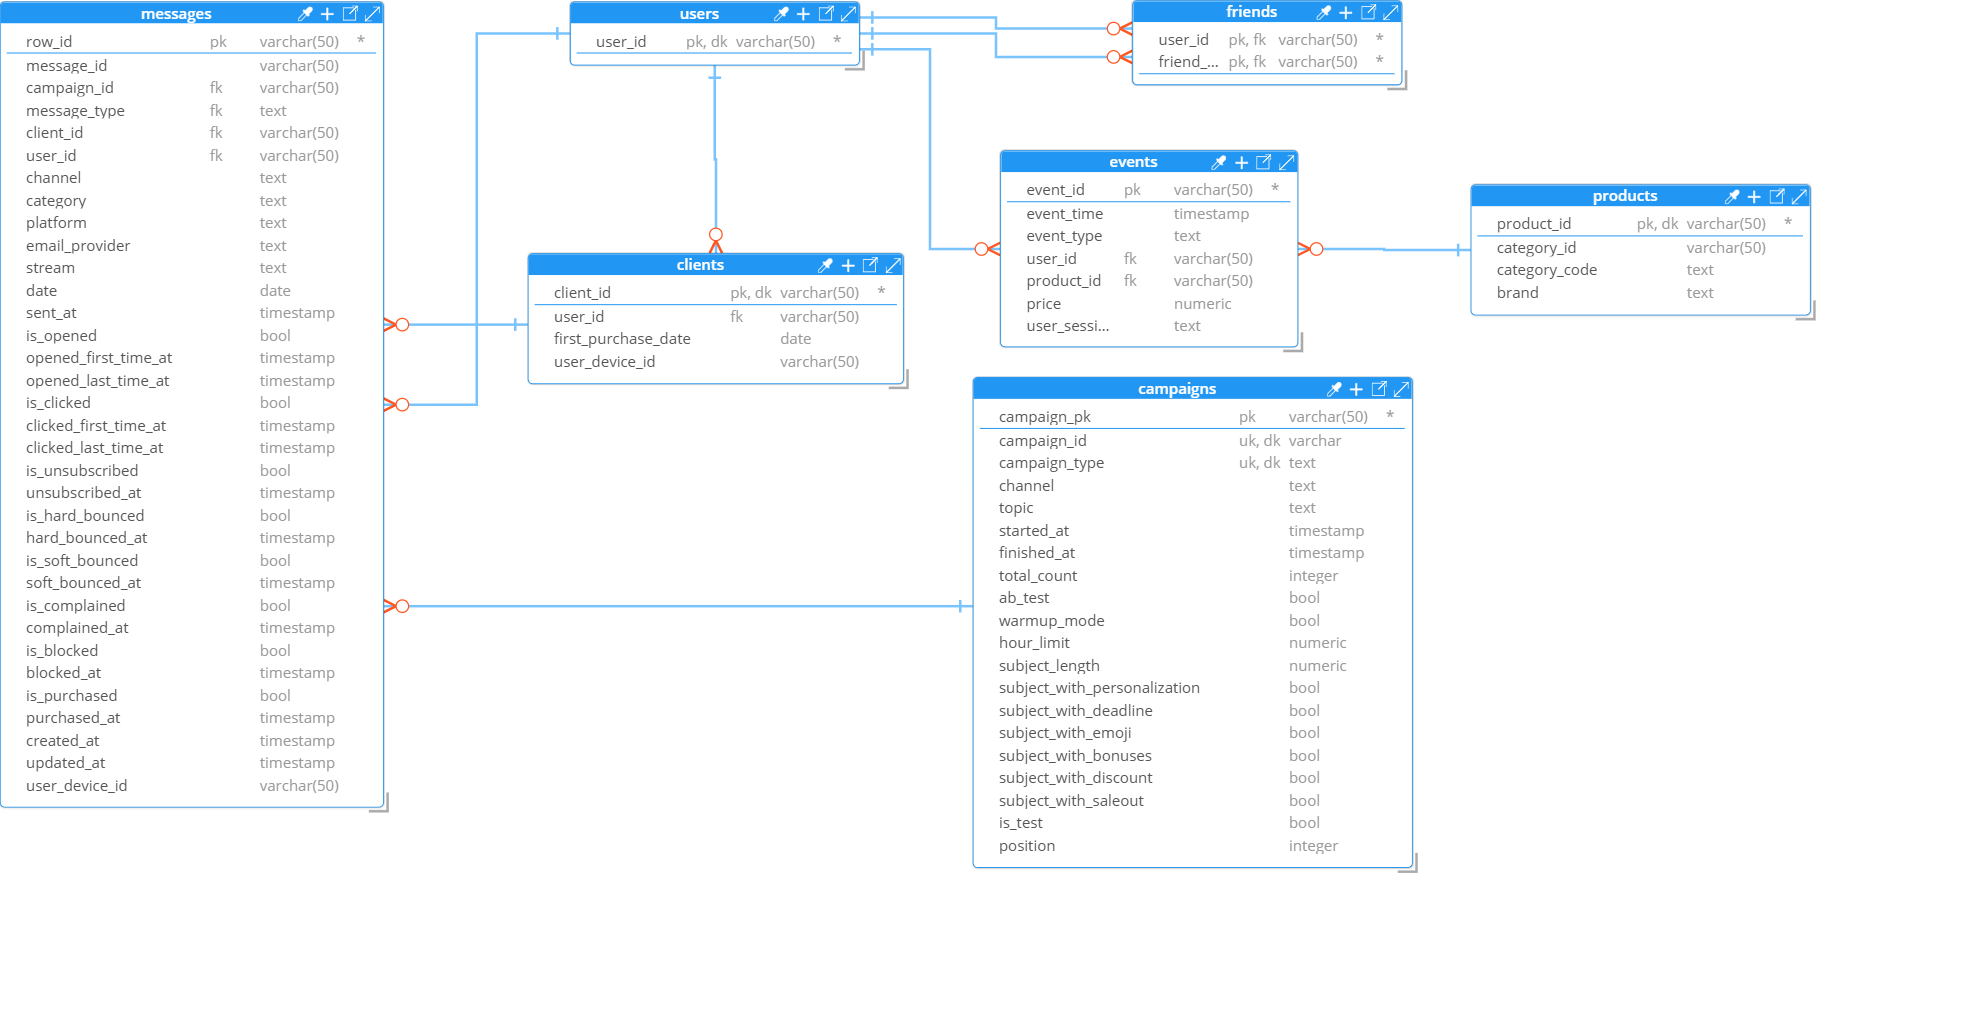
\includegraphics[width=0.95\textwidth]{screenshots/psql_data_model.png}
    \caption{PostgreSQL data model}
\end{figure}

\subsection{MongoDB Data Model}
The MongoDB model was implemented in \texttt{scripts/load\_data\_mongodb.js}. A document model was chosen to reduce the need for many joins and to keep related values together inside documents when that made sense.

The main MongoDB collections are:
\begin{itemize}
    \item \texttt{users},
    \item \texttt{clients},
    \item \texttt{products},
    \item \texttt{events},
    \item \texttt{campaigns},
    \item \texttt{messages},
    \item \texttt{friendships}.
\end{itemize}

Some values were grouped into sub-documents. For example, campaign information inside messages is stored as \texttt{campaign\_ref}, and message actions are stored in an \texttt{engagement} object. Indexes were added for fields such as user IDs, product IDs, campaign keys, and dates. This design helped MongoDB perform well on some tasks, especially the text search task.

\begin{figure}[htbp]
    \centering
    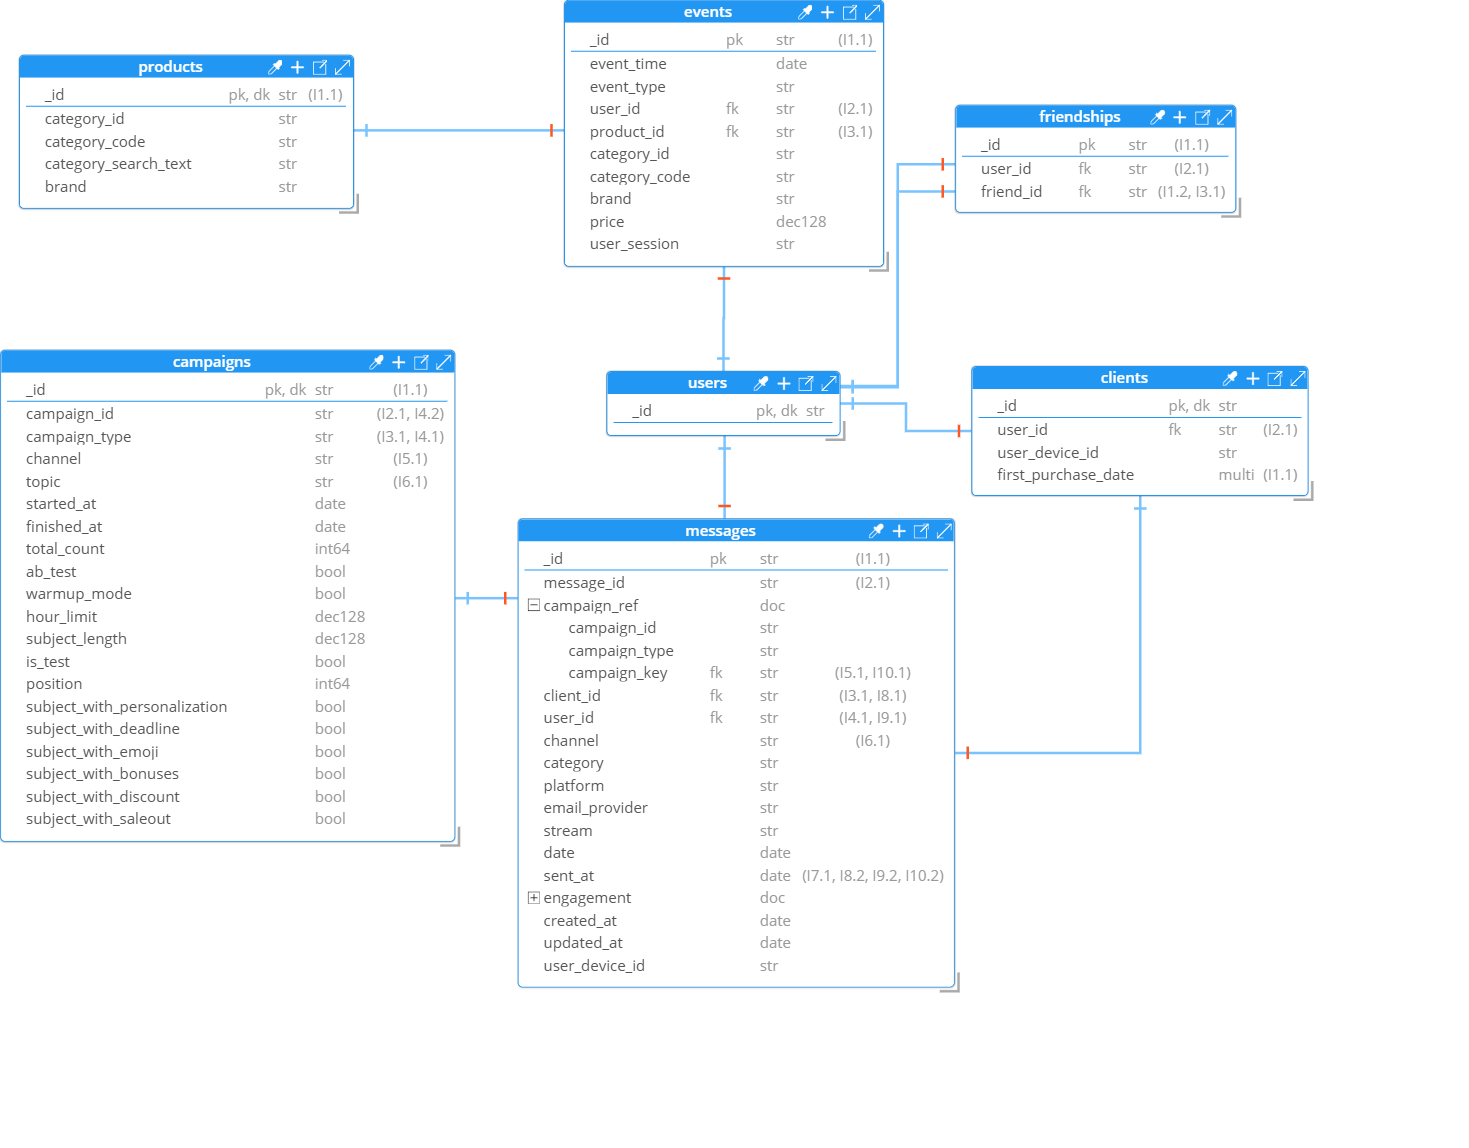
\includegraphics[width=0.95\textwidth]{screenshots/mongo_db_schema.png}
    \caption{MongoDB data model}
\end{figure}

\subsection{Neo4j Data Model}
The graph model was implemented in \texttt{scripts/load\_data\_graph.cypherl}. The design uses graph nodes such as \texttt{User}, \texttt{Client}, \texttt{Campaign}, \texttt{Message}, \texttt{Product}, and \texttt{Category}, with relationships between them.

This model is a good fit for friendship links and recommendation tasks because social connections are first-class relations in a graph database. However, during the work I faced technical issues with Neo4j. Because of that, Neo4j was modeled and prepared, but I did not complete the data analysis and benchmark tasks for it. For this reason, the experimental results in this report focus on PostgreSQL and MongoDB.

\begin{figure}[htbp]
    \centering
    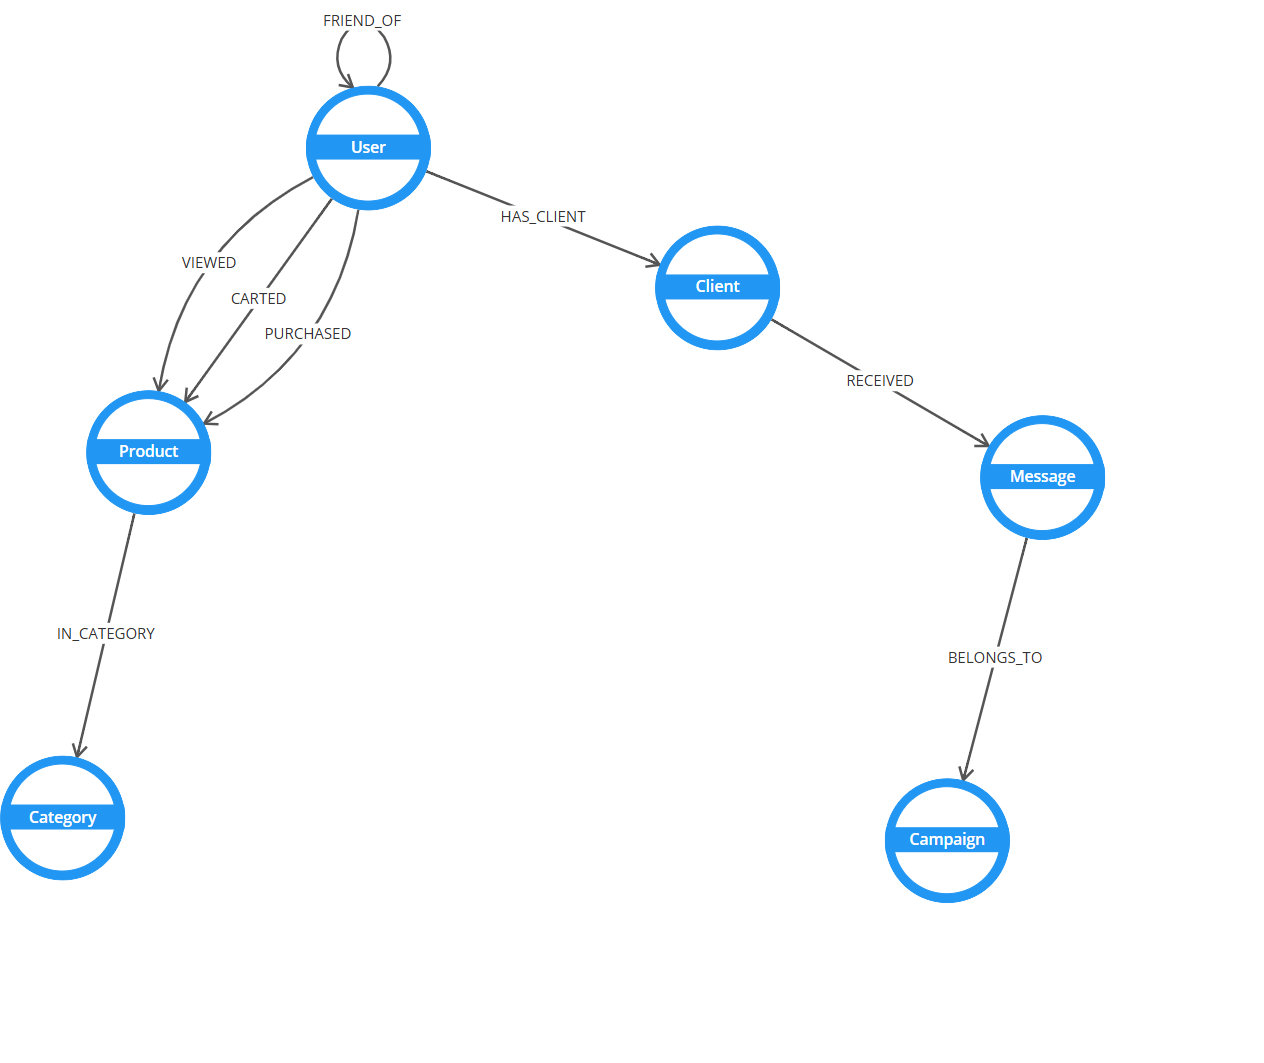
\includegraphics[width=0.95\textwidth]{screenshots/neo4j_data_model.png}
    \caption{Neo4j data model}
\end{figure}

\section{Experimental Results}
\subsection{Analysis Tasks}
The analysis was implemented with Python clients in:
\begin{itemize}
    \item \texttt{scripts/analyze\_psql.py},
    \item \texttt{scripts/analyze\_mongodb.py}.
\end{itemize}

The full query files are:
\begin{itemize}
    \item \texttt{scripts/q1.sql} and \texttt{scripts/q1.js},
    \item \texttt{scripts/q2.sql} and \texttt{scripts/q2.js},
    \item \texttt{scripts/q3.sql} and \texttt{scripts/q3.js}.
\end{itemize}

\subsubsection{Q1: Did campaigns attract purchases?}
Q1 studies whether campaigns led users to purchases. The query first groups messages by campaign and user, then checks which users purchased. After that, it uses the friendship data to find how many purchasers also had at least one friend who purchased in the same campaign. This gives a social support signal.

Both PostgreSQL and MongoDB returned the same top 20 campaign results. The strongest conversion rates were mostly from transactional email campaigns. The best result was campaign \texttt{33} with topic \texttt{order pickup still pending}, with 297 recipients, 7 purchasers, and a conversion rate of 2.36\%. Another strong example was campaign \texttt{32} with topic \texttt{order ready for pickup}, which had 356 purchasers and a small but visible social support share of 1.12\%.

This suggests that transactional campaigns were more effective than bulk campaigns in this dataset. It also suggests that social links may help in some cases, but the effect is not large in most of the top campaigns.

\begin{table}[htbp]
    \centering
    \caption{Q1 execution summary}
    \begin{tabular}{lcc}
        \hline
        Database & Time (sec) & Rows returned \\
        \hline
        PostgreSQL & 18.24 & 20 \\
        MongoDB & 237.08 & 20 \\
        \hline
    \end{tabular}
\end{table}

\subsubsection{Q2: Personalized product recommendation}
Q2 builds product recommendations for the home page. The idea is simple: take the top 100 active users, look at the products their friends interacted with, give a higher weight to purchases and cart actions, remove products that the target user already touched, and keep the top 5 products for each target user.

Both PostgreSQL and MongoDB returned 140 recommendation rows, which means the logic was consistent between the two systems. One clear example is user \texttt{550133755}, for whom product \texttt{1005124} had the highest score of 59 based on 37 friend interactions. Many top recommendations were smartphones and electronics products, which shows that these categories were very active in the dataset.

The result is useful for the business because it gives a practical way to show social-based recommendations on the home page.

\begin{table}[htbp]
    \centering
    \caption{Q2 execution summary}
    \begin{tabular}{lcc}
        \hline
        Database & Time (sec) & Rows returned \\
        \hline
        PostgreSQL & 4.07 & 140 \\
        MongoDB & 3.41 & 140 \\
        \hline
    \end{tabular}
\end{table}

\subsubsection{Q3: Full-text search on top product categories}
Q3 takes the top recommended products from Q2, extracts common keywords from their \texttt{category\_code}, and then searches products using these keywords. In MongoDB, the keywords used were \texttt{appliances}, \texttt{electronics}, and \texttt{smartphone}. MongoDB returned 60 rows for this task and did it very fast.

In PostgreSQL, the stored analysis result for Q3 returned 0 rows. So, for this dataset and implementation, the MongoDB text search gave useful output, while the PostgreSQL version did not return matching products in the saved run. This is an important difference between the two systems in this project.

\begin{table}[htbp]
    \centering
    \caption{Q3 execution summary}
    \begin{tabular}{lcc}
        \hline
        Database & Time (sec) & Rows returned \\
        \hline
        PostgreSQL & 3.75 & 0 \\
        MongoDB & 0.50 & 60 \\
        \hline
    \end{tabular}
\end{table}

\subsection{Benchmarking}
The benchmark data was saved in:
\begin{itemize}
    \item \texttt{benchmark\_results/postgres\_results.csv},
    \item \texttt{benchmark\_results/mongo\_results.csv}.
\end{itemize}

According to the assignment, each query should be run 5 times. This was completed for PostgreSQL. For MongoDB, I ran each query only one time because the first query was very slow on my laptop. This limitation is important, so the MongoDB benchmark numbers should be read with care.

\subsubsection{Raw benchmark results}
\begin{table}[htbp]
    \centering
    \caption{Raw benchmark times for PostgreSQL}
    \begin{tabular}{lccccc}
        \hline
        Query & Run 1 & Run 2 & Run 3 & Run 4 & Run 5 \\
        \hline
        Q1 & 36686.850 & 47662.177 & 23926.330 & 16823.853 & 15065.040 \\
        Q2 & 5485.536 & 3507.523 & 3526.006 & 3806.173 & 3713.116 \\
        Q3 & 4206.594 & 4181.127 & 4478.622 & 4828.611 & 4522.320 \\
        \hline
    \end{tabular}
\end{table}

\begin{table}[htbp]
    \centering
    \caption{Raw benchmark times for MongoDB}
    \begin{tabular}{lcc}
        \hline
        Query & Run 1 & Note \\
        \hline
        Q1 & 227880.041 & only one run \\
        Q2 & 3833.373 & only one run \\
        Q3 & 290.049 & only one run \\
        \hline
    \end{tabular}
\end{table}

\subsubsection{Average and standard deviation}
\begin{table}[htbp]
    \centering
    \caption{Benchmark summary statistics}
    \begin{tabular}{llccc}
        \hline
        Database & Query & Runs & Average (ms) & Std. dev. (ms) \\
        \hline
        PostgreSQL & Q1 & 5 & 28032.850 & 13882.286 \\
        PostgreSQL & Q2 & 5 & 4007.671 & 835.703 \\
        PostgreSQL & Q3 & 5 & 4443.455 & 264.915 \\
        MongoDB & Q1 & 1 & 227880.041 & 0.000 \\
        MongoDB & Q2 & 1 & 3833.373 & 0.000 \\
        MongoDB & Q3 & 1 & 290.049 & 0.000 \\
        \hline
    \end{tabular}
\end{table}

The MongoDB standard deviation is zero only because there was one run, not because the performance is perfectly stable.

\subsubsection{Execution time chart}
\begin{figure}[htbp]
    \centering
    \fbox{\parbox{0.9\textwidth}{
    \textbf{Average execution times (ms)}\\
    PostgreSQL: Q1 = 28032.850, Q2 = 4007.671, Q3 = 4443.455\\
    MongoDB: Q1 = 227880.041, Q2 = 3833.373, Q3 = 290.049
    }}
    \caption{Text summary of average query execution times}
\end{figure}

\subsubsection{Benchmark screenshots}
\begin{figure}[htbp]
    \centering
    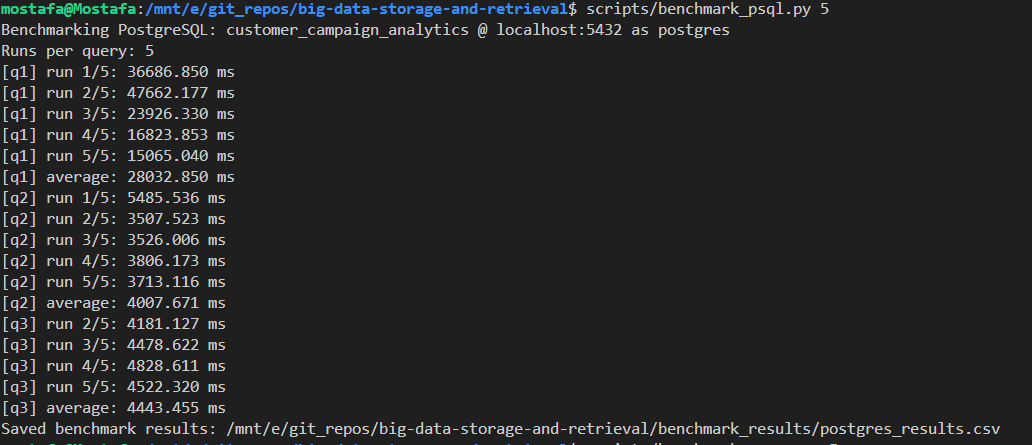
\includegraphics[width=0.9\textwidth]{screenshots/benchmark_psql_results.png}
    \caption{PostgreSQL benchmark screenshot}
\end{figure}

\begin{figure}[htbp]
    \centering
    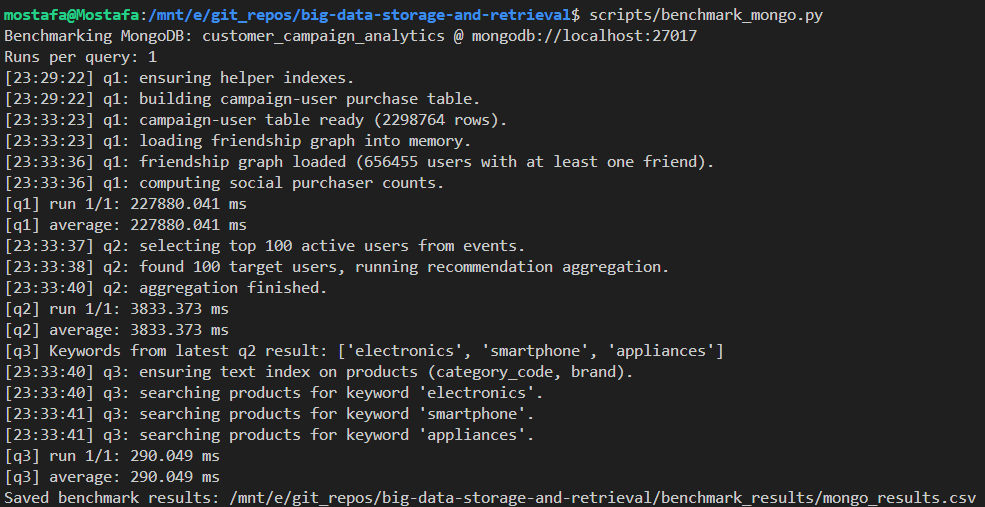
\includegraphics[width=0.9\textwidth]{screenshots/benchmark_mongodb_results.png}
    \caption{MongoDB benchmark screenshot}
\end{figure}

\section{Discussion}
The results show clear strengths and weaknesses for the two tested systems.

PostgreSQL was strong for structured relational analysis. Its schema was normalized, clear, and stable. Q1 and Q2 worked correctly, and the benchmark results were based on five runs, which gives a more reliable view of its performance. The main weakness in this work was Q3, where the saved run returned no rows.

MongoDB was flexible and performed very well for the text search task. Q3 was especially strong in MongoDB, both in result quality and speed. Q2 was also slightly faster than PostgreSQL. However, MongoDB had a major weakness in Q1. That query needed a large amount of processing over messages and friendship links, and on the test laptop it was much slower than PostgreSQL.

The campaign analysis also gives a business insight. Transactional email campaigns had the best conversion rates in the top results. Bulk campaigns appeared in the ranking, but they were not the strongest ones. The social support signal was present, but usually small, so it should be treated as an extra feature and not the only rule for future targeting.

Neo4j is still worth mentioning. In theory, it is a natural choice for friendship-based recommendation because graph traversal fits that problem well. Still, the technical issues I faced meant I could not finish the Neo4j analysis and benchmark stages. Because of that, I cannot make a fair performance comparison for Neo4j in this report.

\section{Conclusion}
In this assignment, three data models were built for the same e-commerce dataset. PostgreSQL and MongoDB were fully used for the analysis tasks, while Neo4j was modeled but not fully tested because of technical issues. PostgreSQL gave better stability and much better Q1 performance. MongoDB gave the best Q3 result and the fastest text search. Based on the completed experiments, PostgreSQL looks like the safer general choice for this workload, while MongoDB is a strong option when flexible document storage and text search are important.

\end{document}
